\documentclass[svgnames,11pt]{beamer}
\input{/home/tof/Documents/Cozy/latex-include/preambule_commun.tex}
\input{/home/tof/Documents/Cozy/latex-include/preambule_beamer.tex}
%\usepackage{pgfpages} \setbeameroption{show notes on second screen=left}
\author[]{Christophe Viroulaud}
\title{Développer un regard réfléchi\\sur les réseaux sociaux}
\date{\framebox{\textbf{ResSoc 03}}}
%\logo{}
\institute{Seconde - SNT}

\begin{document}
\begin{frame}
\titlepage
\end{frame}
\begin{frame}

    Étienne Klein, philosophe des sciences, identifie quatre biais du comportement humain.
    \begin{framed}
        \centering Les réseaux sociaux utilisent-ils les failles du comportement humain pour se développer?
    \end{framed}
\end{frame}
\begin{frame}
    \frametitle{}

    \begin{aretenir}[Biais 1]
    \centering On a tendance à davantage croire une thèse qui nous plaît plutôt qu'une qui nous déplaît.
    \end{aretenir}
    \note[item]{Commenter}
    \note[item]{Exemples?}
\end{frame}
\begin{frame}
    \frametitle{}

    \begin{activite}
    \begin{enumerate}
        \item Donner la définition d'un \textbf{algorithme de recommandation}.
        \item Quels sites ou réseaux utilisent ce type d'algorithme? Lesquels ne les utilisent pas?
    \end{enumerate}
    \end{activite}
\note{Wikipedia n'utilise pas: estime que ça serait un filtrage d'informations}
\end{frame}
\begin{frame}
    \frametitle{}

    \begin{aretenir}[Biais 2]
    \centering On a tendance à croire une chose vraie si on l'a lue ou entendue.
    \end{aretenir}
\note{Fake news se diffuse 6 fois + vite}
\end{frame}
\begin{frame}
    \frametitle{}
\begin{aretenir}[Proposition]
    \centering Les fausses informations se propagent six fois plus vite que les vraies.
\end{aretenir}
    \begin{center}
    \centering
    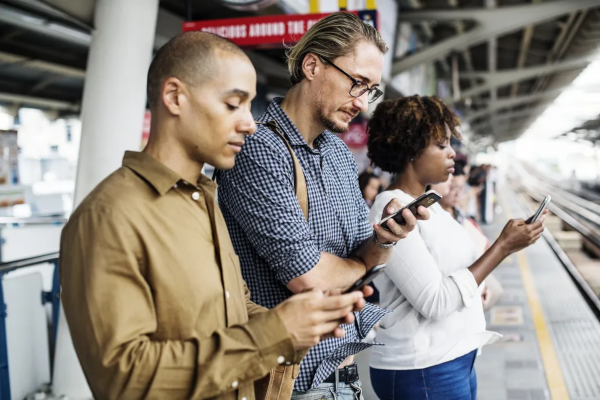
\includegraphics[width=6cm]{ressources/fakenews.png}
    \captionof{figure}{La plupart des usagers des réseaux sociaux partagent les infos sans même les avoir lues\dots}
    \label{IMG}
    \end{center}

\end{frame}
\begin{frame}
    \frametitle{}
\begin{activite}
\begin{enumerate}
    \item Lire l'article \url{https://tinyurl.com/info1mai}
    \item Commenter.
\end{enumerate}
\end{activite}
    

\end{frame}
\begin{frame}
    \frametitle{}

    \begin{activite}
        \begin{enumerate}
            \item Lire l'article \url{https://tinyurl.com/sixfois}
            \item D'où est tirée l'information?
            \item Peut-on considérer l'information fiable? Pour quelle(s) raison(s)?
            \item Quelle semble être la conclusion de cette étude?
        \end{enumerate}
        \end{activite}

\end{frame}
\begin{frame}
    \frametitle{}

    \begin{aretenir}[Biais 3]
    \centering On a tendance à parler avec assurance de sujets que l'on ne connaît pas.
    \end{aretenir}
\note{influenceur: rappeur platiste; booba}
\end{frame}
\begin{frame}
    \frametitle{}
\begin{activite}
\begin{enumerate}
    \item Écouter l'émission \href{https://www.franceinter.fr/embed/player/aod/8d4e5c50-df6a-4189-a4a3-3453bf875477}{Antidote - Booba}
    \item Regarder la vidéo \href{https://www.sciencesetavenir.fr/videos/le-rappeur-qui-croyait-que-la-terre-etait-plate-a-definitivement-perdu-la-partie_l3vzx8}{Le rappeur B.o.B}
    \item Définir l'activité et les limites d'un \textbf{influenceur}.
\end{enumerate}
\end{activite}
    

\end{frame}
\begin{frame}
    \frametitle{}

    \begin{aretenir}[Extrait Midi Libre du 13/11/2020]
    \centering \emph{L'ex-candidate des Marseillais, Kim Glow, a fait polémique mercredi 11 novembre en dénonçant les vaccins à venir contre le Covid-19. Dans une vidéo publiée sur Instagram, la jeune femme annonce que ces vaccins contiendront des puces pour contrôler la population. }
    \end{aretenir}
\begin{center}
\centering

\includegraphics[width=6cm]{ressources/kimglow.jpeg}
\end{center}
\end{frame}
\begin{frame}
    \frametitle{}

    \begin{aretenir}[Biais 4]
    \centering On accorde une très grande confiance à notre intuition personnelle.
    \end{aretenir}
\note{questionnaire}
\end{frame}
\begin{frame}
    \frametitle{}

    \begin{activite}
    Dans le lycée connecté:
    \begin{itemize}
        \item se rendre dans l'application \textbf{formulaire},
        \item répondre au formulaire \textbf{le bon sens}
    \end{itemize}
    \end{activite}

\end{frame}
\begin{frame}
    \frametitle{}

\begin{activite}
    Écrire un résumé (20 lignes maximum) rassemblant les conclusions établies par la classe lors de la séquence, à propos du comportement qu'il peut être important de suivre sur les réseaux sociaux. Le texte s'attachera à ne pas décrire uniquement une vision alarmiste de ce mode de communication.
    \end{activite}

\end{frame}
\end{document}